\documentclass[11pt, a4paper]{article}
\usepackage[czech]{babel}
\usepackage[utf8]{inputenc}
\usepackage{a4wide,color,graphicx,listings}

\title{\textbf{Jabber dungeon}}
\author{Michal Staruch\\
		Ondřej Hlavatý\\
		Petr Mánek}
\date{}

\def\class#1{\emph{#1}}
\def\jid{\texttt{dungeon@eideo.cz}}
\newenvironment{example}%
{\smallskip\noindent\ignorespaces\obeylines\tt}%
{\smallskip\par\noindent
\ignorespacesafterend}

\def\user{\textcolor{blue}{$<$user$>$ }}
\def\dung{\textcolor{red}{$<$dungeon$>$ }}
\lstset{
  keepspaces=true,
  basicstyle=\footnotesize,
  language=C++,
  tabsize=4,
  showspaces=false,
  showstringspaces=false
}

\begin{document}

\maketitle

\section{Zadání}

Projekt byl zadán jako zápočtový program na MFF UK. Cílem bylo vytvořit herní systém textové adventury, kterou bude možno hrát přes komunikační síť Jabber. Samotná adventura by měla být rozumně ovladatelná textovými příkazy a komunikovat s uživatelem přirozeným jazykem - v angličtině. Herní svět je společný pro všechny hráče, kteří se v něm pohybují nezávisle.

Jako jazyk implementace byl zvolen \texttt{C++}. Součet schopností programovat v týmu byl pro tento jazyk největší, a zároveň je vhodný pro objektový návrh.

\section{Základní návrh}

Srdcem celé hry jsou objekty \class{GameManager} a \class{ActionQueue}. Většinu informací přenáší objekty \class{ActionDescriptor} (AD). Komunikace s uživatelem probíhá skrz \class{Driver}.

Nejprve, jak vypadá životní cyklus \class{ActionDescriptoru}.
\begin{figure}[htp]
\centering
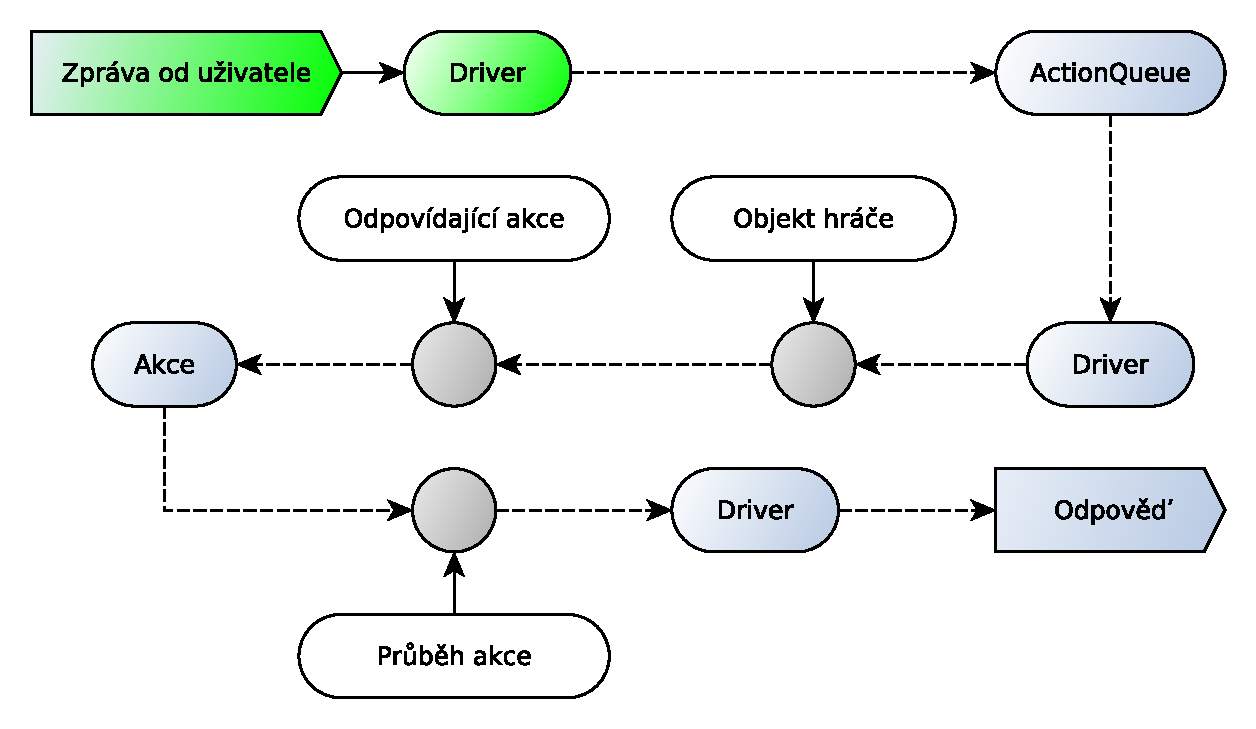
\includegraphics[scale=0.6]{AD-lifecycle.pdf}
\caption{Životní cyklus \class{AD}}
\label{ad-lifecycle}
\end{figure}

Každý běžící \class{Driver} má své vlastní vlákno (na obrázku zeleně), odlišné od hlavního herního vlákna (modře). V okamžiku přijetí zprávy vytvoří driver objekt AD nebo jeho potomka. Uloží si do něj všechny potřebné informace pro další zpracování (odesílatele, text zprávy atp.) a  zařadí jej do fronty v ActionQueue. Ta pak ve svém vlákně přiděluje čas na zpracování akce postupně a zajišťuje tím atomicitu operací \uv{zadarmo}. Když na tuto akci dojde řada, tak se teprve zjišťuje Driver co vlastně má provést. Jako první sváže akci s herním objektem uživatele - v tomto vlákně již má přístup k databázi. Poté z věcí v okolí sežene seznam proveditelných akcí a zjistí, která odpovídá vstupnímu textu. Jakmile je akce svázána, předá se řízení dané akci. Ta provede změny v herním světě a vloží do AD informace potřebné k sestavení odpovědi.

Stručně pár dalších důležitých tříd v návrhu:

\paragraph{GameManager (GM)} zprostředkovává samotný přístup k herním objektům a světu. Izoluje herní mechanismy od úložiště informací, zpřístupňuje některé zkratky.

\paragraph{ObjectPointer (OP)} Během načítání herních objektů se může stát, že GM odstraní z paměti jiný načtený objekt z důvodu úspory paměti. OP umožňuje při přístupu objekt nechat znovu načíst.

\paragraph{Driver} Implementovány jsou aktuálně \class{TextDriver}, obsluhující zprávy textového charakteru, a jeho potomci \class{ConsoleDriver} a \class{JabberDriver}. Jeden umožňuje ovládat postavu ze standartního vstupu a zprávy vypisovat na standartní výstup, druhý se přihlašuje jako jabber klient s adresou \jid a komunikuje pomocí XMPP.

\paragraph{Action} Její potomci reprezentují proveditelnou akci. Obsahuje zejména metodu \texttt{commit}, která spustí provedení akce.

\paragraph{IObject} Každý objekt ve hře implementuje toto rozhraní. Obsahuje metody pro zjišťování informací o objektu, persistenci vlastností a udržování relací.

\paragraph{ThorsHammer} Speciální herní objekt. Kdo jej vlastní, má přístup k administrátorským funkcím hry.

\section{Reprezentace herního světa}

Každý objekt ve hře má svůj unikátní textový identifikátor a je instancí třídy implementující rozhraní IObject. Téměř každý objekt také implementuje rozhraní \class{IDescriptable}, které poskytuje objektu název a rozsáhlejší popis. 

Objekty mezi sebou uchovávají relace, což jsou orientované hrany s daným typem. Mezi dvěma objekty může existovat pouze jedna relace od každého typu a směru.

\subsection{Persistence}

Jednotlivé vlastnosti objektů i relace jsou uchovávány v databázi. Relace jsou uložitelné jednoduše, na vlastnosti objektů má každý potomek IObjectu metodu \texttt{registerProperties}. V ní ohlásí, jaké vlastnosti má. Tyto data využije objekt \class{Archiver} a serializuje data do binárního streamu. Ten se pak může do databáze uložit. Stejnou metodou se pak data do objektu dají načíst zpět -- obrátí se směr Archiveru, a ten místo čtení hodnoty nastaví. Neví přitom nic o tom, jaké hodnoty ukládá, stačí mu k tomu typ.

To ale není jediné využití této metody. Dá se ji podstrčit libovolný objekt implementující \class{IPropertyStorage}, například administrátorský nástroj \class{PropertyEditor}, který je využije k pohodlné úpravě všech vlastností objektu přes libovolné herní rozhraní.

Instance objektů by se vytvářeli snadněji v nějakém dynamickém jazyce

\subsection{Uchovávání v paměti}

Herní svět může bý snadno docela veliký, proto jej nikdy nechceme načítat do paměti celý. Všechny herní objekty se proto načítají na vyžádání v době potřeby, kde to jde tak se používá pouze id objektu, předávané pomocí OP. Pro uchovávání již načtených objektů používáme Splay strom, protože umožňuje rychle přistupovat k objektům, které se používají hodně.

V současné chvíli to není implementováno, ale je možné tento strom upravit tak, aby objekty v určité hloubce (tedy dlouho nepoužité) zahazoval, a tím uvolnil paměť.

Z databáze načítá objekty \class{ObjectLoader}, ke čtení vlastností se využívá Archiveru. \class{DatabaseHandler} uzavírá práci s databází, používáme SQLite.

\section{Herní objekty a akce}

Jak už bylo řečeno, všechny objekty dědí IObject a zpravidla také IDescriptable. Základní vlastností herního objektu je schopnost zjistit akce dostupné na tomto objektu. Tak je dosaženo maximální flexibility světa. Není třeba mít na jednom místě seznam všeho co lze kdykoli provést, a v různém kontextu se mohou stejné zprávy vyhodnotit různě. 

Při zpracovávání akce se v jednu chvíli zjistí akce na všech objektech v okolí uživatele, a postupně se na nich spouští metoda \texttt{matchCommand}. Jakmile se první akce k příkazu přihlásí, je provedena a na ostatní se již nedostane.

Dalšími obecnými typy objektů jsou:

\paragraph{Alive, Human} Reprezentují žívé objekty a uživatele. Každý živý objekt má své umístění a zbývající počet životů. Dostupně akce na těchto objektech jsou zejména týkající se pouze daného uživatele. Tj. zjišťující aktuální stav, různé nápovědy, přejmenování atp.

\paragraph{Creature} Reprezentují všechny objekty, na které se dá útočit, tedy všechna monstra a živočichy. Akce na tento objekt je zejména attack.

\paragraph{Item} Cokoli, co jde uchopit. Objekt samotný nemá akce, ale má vlastnosti \texttt{size} a \texttt{weight}, udávající velikost a váhu objektu.

\paragraph{Wearable} Cokoli, co jde použít jako část oděvu. Tento objekt používají zbraně a různé typy brnění. Umožňuje objektům měnit bojové vlastnosti postav (útočné číslo, obranné číslo, počet životů)

\paragraph{Inventory} Potomek Wearable, přidává navíc akci drop a umožňuje v sobě ukládat předměty.

\paragraph{Location} Reprezentuje lokaci, ve které se ostatní objekty nacházejí. Tyto lokace jsou buď místnosti, které jsou s ostatními místnostmi spojeny dveřmi, nebo truhly, které obsahují předměty. Akce na lokaci jsou zejména průzkumné. 

\paragraph{Door} Jedno nebo obousměrný teleportační tunel mezi dvěma lokacemi. Akcí na tomto objektu je průchod skrz.

\paragraph{Crafter} Speciální objekt, který je používán pro tvorbu věcí. Udržuje v sobě objekty \class{Recipe}, které říkají, jaké věci umí \class{Crafter} vyrobit. Ve hře se vyskytuje například jako kovadlina.

\paragraph{Resource} Potomek třídy \class{Item}, reprezentuje věci, které se seskupují, tedy například peníze, nebo materiály pro \class{Crafter}.

\subsection{Parametrizované akce}

Velmi častým požadavkem je, aby akce měla nějaký parametr. Například když v místnosti leží tři lektvary, je potřeba určit který z nich se má akcí vypít. Tento problém důstojně řeší \class{MultiTargetAction} (MTA). Objekt vytvoří instanci MTA, a do seznamu cílů přidá sám sebe nebo i jiné objekty, na které lze akci zacílit. Při přidávání do seznamu se podle identifikátoru zjistí, že stejný druh akce již v seznamu je, a seznamy cílů se spojí v jeden. Akce si potom při spuštění vybere ze seznamu ten objekt, který nejlépe odpovídá zadanému textu.

Zároveň, pokud je v místnosti pouze jeden lektvar, pak spuštění akce vypije právě ten jeden lektvar i bez bližšího určení.

Při výběru objektů se porovnává editační vzdálenost (Damerau-Levenshteinova) názvu objektu od zadaného textu. Při počítání vzdálenosti je změna znaku pocítána jako větší úprava, než přidání či odebrání. Proto je větší šance, že přidání neurčujících slov (členů, zájmen) a naopak nespecifikování částí názvu (bližší popisy) tolik neovlivní volbu.

\section{Další (nejen) herní mechanismy}

\subsection{Skupinový popis}

Aby hraní působilo přirozeněji, popisovatelné objekty se umí sdružit podle typu a vypsat jednotný popis za všechny. Funkcionalitu zajišťuje třída \class{ObjectGroup}. Výpis pak může vypadat třeba takto:

\begin{example}
\dung You see Piece of wood and Stone. There lies Red potion, Green
potion and Blue potion. 
\end{example}

\subsection{Dialogy}
\label{dialogs}
Zpočátku vypadal hra striktně podle režimu příkaz -- odpověď, a hra připomínala spíše příkazový řádek\footnote{Z čehož vznikly aliasy pro akce, např. \texttt{cd} pro průchod dveřmi :)}. Toto schéma rozbíjí mechanismus dialogu:

\begin{example}
\user rename myself
\dung Well then, what do you want your new name to be?
\user New name
\dung OK. You shall now be called New name. I'm just curious, why did 
you change your name?
\user Because I wanted to show, how dialogs work.
\dung Interesting. Now, back to the dungeon!
\end{example}

\subsection{Boj}
\label{combat}
Systém boje vznikl krátce po vzniku dialogů a hojně jich využívá. Každá instance třídy \class{Creature} přidá akci \texttt{attack}, která inicializuje boj. Po zavolání akce \texttt{attack} se pustí obslužná metoda, která vždy provede požadovanou akci a v dialogu se zeptá uživatele, co dělat dále. Pokud hráč dosáhne 0 životů, zemře, pokud dosáhne 0 životů \class{Creature}, dostane se do stavu \texttt{Dying}. V tomto stavu je přidána akce kill, která dorazí příšeru.

\subsection{Smrt}

Smrt nastane, pokud životy hráče nebo nepřátel dosáhnou nuly. Metoda \texttt{changeHp}, která se stará o změnu počtu životů automaticky zavolá obslužnou proceduru \texttt{die}. V případě třídy \class{Human} procedura změní stav hráče na mrtvého, zakáže mu většinu akcí kromě některých výjimek a znemožní mu hrát po stanovený interval. Po uplynutí toho intervalu se může hráč akcí \texttt{respawn} oživit, při oživení je přemístěn do poslední místnostni s flagem \texttt{respawnable}, kterou hráč navštívil. V případě třídy \class{Creature} je na zem puštěna odměna za zabití (pokud nějaká je) a instanci se naplánuje automatický respawn, který je kontrolován (a popřípadě proveden) při zjišťování akcí.

\subsection{Pasti}

% TODO Napsat to a zadokumentovat

\section{Programová část}

V této kapitole bychom chtěli vypíchnout některé části kódu, které se nám líbí, jsou zajímavé, nebo se k nim váže nějaká příhoda.

\subsection{Logování}

Podstatnou částí systému, na kterou jsme patřičně hrdí, je logovací mechanismus.

% TODO Petře, vyvětrej svou chlubnou plíci :)

\subsection{Výběr náhodné zprávy}

Pro ozvláštnění komunikace je dobré nemít všude stejné statické texty, ale výpis trochu měnit.

\begin{example}
\user something
\dung One does not simply ask me to "something".
\user something
\dung I wouldn't do that if I were you. Besides, I can't do that.
\user something
\dung The day may come when I understand "something"{} but it's not 
this day.
\end{example}

\noindent Pro tento účel jsme si napsali utilitku \class{RandomString}, která se používá takto:

\begin{lstlisting}
	return RandomString::get()
		    << "What do you mean \"" + input + "\"?" << endr
		    << "One does not simply ask me to \"" + input + "\"." << endr
		    ...
			<< "This is not the thing you are trying to do." << endr;
\end{lstlisting}

\noindent Třída využívá přetížení operátoru \texttt{<<} a přetypovaní na string.

\subsection{InstanceOf}

Potřeba použití nečeho takového signalizuje chybu v návrhu, ale pokud chceme mít obecný mechanismus práce s objekty, je občas potřeba o obecném \texttt{IObject*} zjistit něco více. Proto se hodí tento operátor. Použití:

\begin{lstlisting}
	Alive* A;
	A->instanceOf(Backpack); // true / false
\end{lstlisting}

\noindent Celá věc funguje trochu magicky, ale hlavně rychle. Pomocí preprocesorových maker se v každém objektu vytvoří virtuální inline funkce \texttt{className} a \texttt{isInstanceOf}. ClassName vrací konstantní řetězec obsahující název třídy -- ten se používá například pro serializaci do databáze. Pro použití s instanceOf se ale počítá jen s ukazatelem na tento řetězec. Pomocí dalších maker se ukázka přepíše takto (s využitím konstanty):

\begin{lstlisting}
	A->isInstanceOf(Backpack::BackpackClassName); // true / false
\end{lstlisting}

\noindent A protože je funkce inline, kompilátor ukázku přepíše například takto:

\begin{lstlisting}
	Alive::AliveClassName == Backpack::BackpackClassName 
		|| IDescriptable::IDescriptableClassName == Backpack::BackpackClassName 
		|| IObject::IObjectClassName == Backpack::BackpackClassName;
\end{lstlisting}

\noindent Celý operátor tedy pouze projde hiearchii volané třídy a porovná ukazatele na tento konstantní řetězec.

\subsection{Dialogy}

O tom jak vypadají dialogy v praxi bylo již psáno v části \ref{dialogs}. Jak se ale dialogy používají? Příklad je celý kód akce na přejmenování uživatele:

\begin{lstlisting}
	*ad << "Well then, what do you want your new name to be?";
	ad->waitForReply([] (ActionDescriptor *ad, string reply) {
		((Human*) ad->getAlive())->setUsername(reply)
				->save();
		*ad << "OK. You shall now be called " 
			<< ad->getAlive()->getName() << ". "
		    << "I'm just curious, why did you change your name?";
	});
	ad->waitForReply([] (ActionDescriptor *ad, string reply) {
		*ad << "Interesting. Now, back to the dungeon!";
	});
\end{lstlisting}

\noindent ActionDescriptor umožňuje zařadit do své vnitřní fronty lambda funkci, která bude reagovat na odpověď uživatele. Pokud AD nemá frontu prázdnou, musí si jej Driver někde zapamatovat a vrátit se k němu při přijetí další zprávy.

Všechny lambda funkce nemusí být vytvořeny hned, dají se vytvářet postupně. Tento zápis je však přehledný, a z kódu je hned vidět jak dialog probíhá. Zároveň je ale možno udělat dialog, který není lineární, nebo třeba není předem známý - například boj.

\subsection{Cloner}

Původní myšlenkou bylo to, že všechny objekty budeme vytvářet ručně a během hry. Postupem času se však ukázalo, že toto není nejlepší nápad a tak jsme hledali způsob, jak objekty vytvářet rychleji.

Nakonec jsme přišli s třídou \class{Cloner}, která využívá vlastnosti objektů a pomocí \class{IPropertyStorage} je schopen je přečíst. Při jejich čtení si je ukládá do své paměti. Po přečtení využije další metodu naší perzistence a tou je \texttt{createObject}, kterou vytvoří čistou kopii objektu. Poté z uloženého seznamu nahraje všechny vlastnosti nového objektu, změní mu \texttt{id} a vrátí tento objekt. Tuto kopii nazýváme \texttt{shallowCopy}

\class{Cloner} umí vytvořit ještě \texttt{deepCopy}, která navíc zkopíruje všechny relace objektu.

Tuto třídu hojně využíváme při vytváření světa ve třídě \class{WorldCreator}, kde nejprve vytvoříme vzory všech objektů a poté už je jenom rozkopírujeme, kde je potřeba.

\section{Ukázky}

Rádi bychom ukázali nějaké naprosto základní ukázky komunikace s programem.

\begin{example}
\user hello
\dung Hi!
\user where am i
\dung You are in Base Camp. Nothing much to be found here, but get
familiar with basic commands - try to type 'help'. There is a wooden
door. You recognize Salmelu and CiTrus. You have a Leather backpack 
with you.
\user go to that wooden door
\dung You are in Equip room. Looks like noone has been there for 
a long time. There is a wooden door. You see Green potion, Blue potion 
and Red potion. 
\user drink the blue potion
\dung You've drunk Blue potion. You've healed 100 hitpoints
\user pick the red potion
\dung You've picked up Red potion.
\user explore
\dung You are in Equip room. Looks like noone has been there for 
a long time. There is a wooden door. You see Green potion lying on the 
ground. You have a Leather backpack with you. There is Red potion.
\user drop the red potion
\dung You've dropped Red potion. 
\end{example}

\end{document}
